\subsection{Implementation}
	From the very beginning on, the \ac{DALPHI} framework was planned as an open source software. The appendix \ref{appendixDalphiDev} includes a further explanation of the development process, including a description of who was involved and who funded the development.

	The software is a WebApp, based on the Ruby on Rails framework.\footnote{Ruby on Rails: \urlWithDate{http://rubyonrails.org/}}
	This offers a modern, flexibel and convenient development environment and the fact that the resulting product is a WebApp satisfies the requirement of making its use platform independent and inherently available to everyone at once having access to the internet and a web browser~\cite{bachle2007ruby}. Thus it belongs to the multi-user class of annotation tools.

	Since the main focus of this work is on the impact of the assistance to human annotators (Section~\ref{sec:results}), its software core (the \ac{MEC}) is treated as a black box, using the \ac{NLTK} as an off-the-shelf \ac{NLP} library.\footnote{\ac{NLTK}: \urlWithDate{http://www.nltk.org/}}

	\subsubsection{Web Service Architecture}
		\label{sec:implementationWSA}
		\ac{DALPHI} should act as a general purpose annotation framework, flexible enough to accommodate many different applications. As such, it is problem agnostic and the core components (\ac{UI}, \ac{ML} component / assistance and a merge service as described in~\ref{dalphiMergeService}) are not supplied.\footnote{At least not all of them: The used components for labeling training data for \ac{NER} tasks are fully open source and may provide a good starting point to create own services for the framework (interface: \urlWithDate{https://github.com/Dalphi/interface-ner_complete} and \ac{ML} and merge service component: \urlWithDate{https://github.com/Dalphi/service-ner_iterate}).}
		The need to write ones own (problem specific) code creates the necessity to make these components as easy to write as possible. We created and open sourced examples of all components and they are easy to adapt to be used in ones own scenarios.\footnote{We provide three examples of an annotation \ac{UI}, for a very basic full paragraph classification with only a few lines of code to a more complex \ac{NER} annotation interface with different user interactions like mouse movements and keyboard shortcuts. Our example iteration service provides the complete classifier for examplatory purposes, but the necessary \ac{DALPHI} \ac{API} calls are written in only one simple file.}
		Instead of including them into a large monolithic code base, these components are accessed using a simple RESTful \ac{API}~\cite{w3crestarch}. This allows users to rapidly prototype their code and does not restrict them to any specific programming language or toolchain; they don't have to leave the environment they are used to. The only requirement is a rather simple HTTP interface and the convention that all transmitted data have to be \ac{JSON}~\cite{bray2014javascript} encoded.

		The assistance system is a stand alone web service. It is called by the \ac{DALPHI} framework after an annotation iteration has finished and the newly annotated passages are already merged back to into the corpus. This (\ac{JSON} encoded) corpus is now sent via an asynchronous HTTP-POST request, together with a unique callback ID, to the web service.\footnote{A unique callback ID is necessary because of the asynchronous request: The data size of the corpus can be that large, that the time of the initial transmission, the processing and the transmission of the answer back to the framework would cause HTTP timeouts. To avoid this, requests are asynchronous and need an identifier to tell the \ac{DALPHI} framework to which request an answer belongs.}
		The web service immediately returns a HTTP success status code after the transmission has ended successfully. It now extracts all the sentences containing at least one annotation and trains an \ac{NER} model using \ac{NLTK} (see Section \ref{sec:nerWithNLTK}). The resulting model is subsequently used to label all the parts of the corpus that have not been annotated by a human. Now the resulting model has all the human made annotations and (hopefully) some more, created by the \ac{NER} model. This annotated corpus is now split up into several \textit{annotation documents} that will be evaluated by (a) human annotator(s) in the next iteration. The web service may order these documents as well: Such an order could define for which documents the algorithm wants human feedback (the \ac{AL} approach, see Section~\ref{sec:conceptionNERatHeart}). Finally these documents are returned to the \ac{DALPHI} framework, using an HTTP-POST response request to the callback url the framework provided with its initial call.

	\subsubsection{\acl{NER} Using \acs{NLTK}}
		\label{sec:nerWithNLTK}
		The assistance web service was developed using the Python programming language.\footnote{Python 3.6.1: \urlWithDate{https://www.python.org/downloads/release/python-361/}}
		The Python community offers an exhaustive set of packages, and a noticeable amount of \ac{NLP} libraries.\footnote{Some of the better known ons are: \ac{NLTK}, TextBlob, Stanford CoreNLP, ...}
		In this case \ac{NLTK}'s \acl{MEC} was used to provide an \ac{NER}~\cite{nltkinfoextract} assistance. Generally, the features of the Named Entity chunker were used as recommended:\footnote{See \ac{NLTK}'s documentation of the \textit{nltk.chunk.named\_entity} class: \urlWithDate{http://www.nltk.org/_modules/nltk/chunk/named_entity.html}}

		\begin{enumerate}
			\item \textit{shape:} Which shape does the current token have? Is it made up of numbers, punctuation, uppercase characters, lowercase characters, mixedcase, other?
			\item \textit{wordlen:} The number of characters of the token.
			\item \textit{prefix3:} The first three chars of the token.
			\item \textit{suffix3:} The last three chars of the token.
			\item \textit{pos:} The \ac{POS} tag, like Noun, Verb, Pronoun, Preposition, ...
			\item \textit{word:} The word itself.
			\item \textit{en-wordlist:} Is the word included in a english dictionary?
			\item \textit{prevtag:} The named entity tag of the previous token.
			\item \textit{prevpos:} The \ac{POS} tag of the previous token.
			\item \textit{nextpos:} The \ac{POS} tag of the next token.
			\item \textit{prevword:} The previous word.
			\item \textit{nextword:} The next word.
			\item \textit{word\+nextpos:} The current token (lowercased), concatenated with the \ac{POS} tag of the following token.
			\item \textit{pos\+prevtag:} The \ac{POS} tag of the current token, concatenated with the named entity tag of the previous token.
			\item \textit{shape\+prevtag:} The shape of the current token, concatenated with the named entity tag of the previous token.
		\end{enumerate}

		\paragraph{Adjustments for German Texts}
		The following adjustments to the feature set were necessary to be able to use the chunker with German texts:

		\begin{enumerate}
			\item A German \ac{POS} tagger was used. \ac{NLTK}'s default provides \ac{POS} tagging for English sentences, which can not be applied to German texts. A suitable tagger was available as open source software via GitHub~\cite{nltkClassifierBasedGermanTagger}.
			\item A German word list was employed. It is provided as open source as well and was created for the GNU Aspell project.~\cite{gnuAspellGermanWordlist}
		\end{enumerate}

		This work is about the effect an \ac{AL} based assistance system has on the performance of human annotators. The working assistance system with an underlying \ac{NER} algorithm is a proof of concept. It shows that the general idea of employing \ac{AL} as an automated annotation assistance actually works. Therefore, the classifier we chose -- despite the availability of more performant alternatives~\cite{benikova2014germeval} -- is a solid, well known (due to its frequent use in other works), as well as easily comprehensible algorithm. It serves as a baseline of what is possible in the field of \ac{NER}.

		\paragraph{Mechanics of the \acl{MEC}}
		\label{sec:algorithmicFoundationMEC}
		The \ac{NER} assistance system was implemented using a \acf{MEC}. Maximum Entropy modeling was first described by E.~T.~Jaynes in 1957~\cite{jaynes1957}. The classifier chooses from a set of labels and assigns each word one of it. Usually the labels are the different entities (person name, organization name, city, geo political entity, ...) concatenated with \textit{beginning} or \textit{inside} to describe each state a word can have~\cite{tjong2003introduction}. For example, Figure~\ref{fig:ambiguousWordPair} shows the term \lqq Washington Redskins\rqq, describing an organization named \lqq Washington Redskins\rqq or a location \lqq Washington\rqq and a following organization \lqq Redskins\rqq.

		\begin{figure}[h]
		  \centering
		  \subfloat[Both words together are the name of an organization.]{{
		    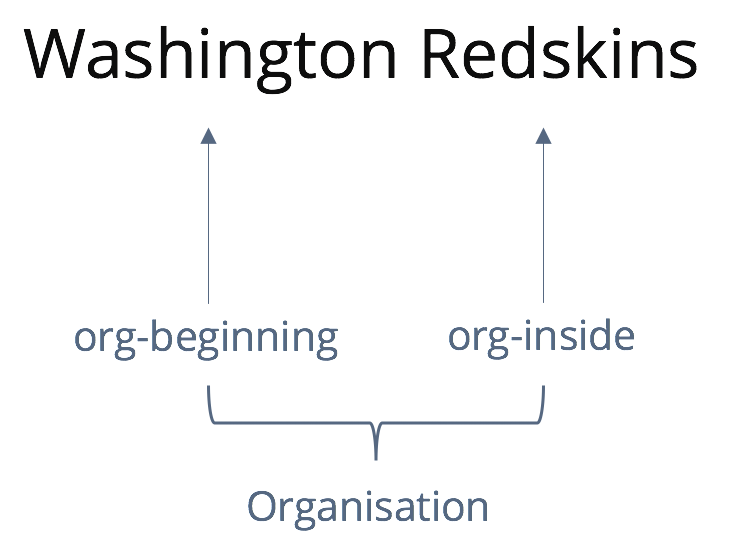
\includegraphics[width=4.5cm]{assets/2/BIOtagsWashingtonRedskins2.png}
		  }}
		  \qquad
		  \subfloat[Each word has a meaning of its own: A location, followed by an organization.]{{
		    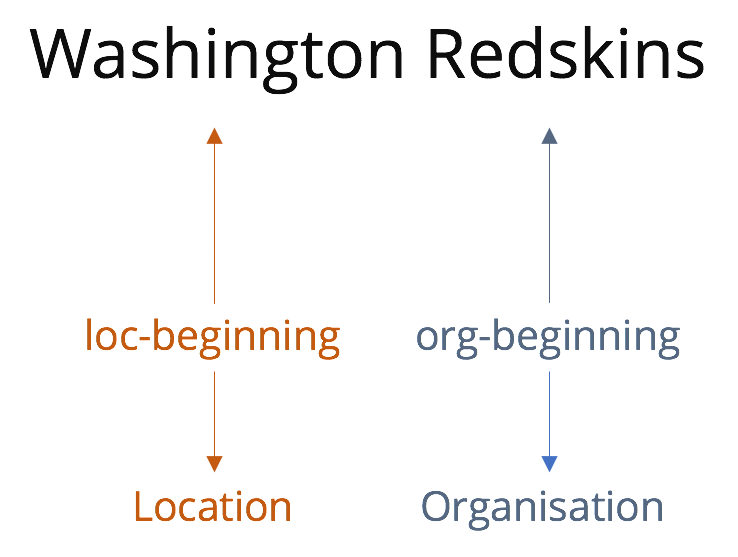
\includegraphics[width=4.5cm]{assets/2/BIOtagsWashingtonRedskins1.png}
		  }}
		  \caption{A word pair example with an ambiguous meaning.}%
		  \label{fig:ambiguousWordPair}%
		\end{figure}

		Only the \textit{beginning} or \textit{inside} suffix of the labels make this clear: Either the labels \textit{organization-beginning} followed by \textit{organization-inside} are used and represent the first example interpretation (\lqq Washington Redskins\rqq), or the labels \textit{location-beginning} followed by \textit{organization-beginning} are used to represent the second interpretation. This way, the beginning / inside suffixes are used for disambiguation. Additionally, an \textit{outside} tag is available to tag words not belonging to any entity. Figure~\ref{fig:NERtaggedBIOexample} provides an example of a complete tagged sentence using this technique.

		\singleFullSizeFig{2/bio-tags-example.png}{A named entity tagged example sentence using the beginning / inside / outside notation.}{NERtaggedBIOexample}

		The maximum entropy classifier builds a model to predict the probability of a label $y$ given an input word $x$, $P(y\ |\ x)$. It is used to answer the question \lqq Which label suits a given input best?\rqq.\footnote{Since this classifier belongs to the class of conditional classifiers it can also be used to ask for the probability of a given label for a given input; but in this case we are interested in the most likely label for each word of the plain, unannotated text.}
		Not every label can always be applied: If the previous word was the beginning of a person's name the current word can not be tagged \textit{location\_inside} since this would require a preceding \textit{location\_beginning}. Instead, in this case, only the tags \textit{person\_inside}, \textit{outside} or all beginning-tags would be possible.

		Several features can be computed for every input word $x$, e.g.~some binary ones like \textit{is the word capitalized?} or \textit{is the word included in a dictionary of the same language?}. Nominal variables may be included in the feature set as well, like a word's \textit{\acf{POS} tag} (the word category like noun, verb, pronoun, ...) or even \textit{the number of characters the word has}. These nominal variables will be converted to vectors of binary values before being applied to the algorithm~\cite{nigam1999using}. This conversion results in relatively large but sparse binary \textit{feature vectors} (sets of all features of an input word).

		Features are represented in functions that can contain logic like the lookup in a dictionary. \(g_i(x, y)\) is an example of such a feature function for an input word $x$:

		\begin{equation*}
		   g_i(x, y) =
		  \begin{cases}
		      1, & \parbox[t]{.6\textwidth}{
		        $x \notin german\_dictionary \wedge y =$ org-beginning
		      }\\
		      0 & \text{otherwise}
		  \end{cases}.
		\end{equation*}

		Here \(i\) indicates the number of the feature and \(german\_dictionary\) in this example is a list of German words. A word that is not included in such a dictionary will most likely be a new word creation and hence it is a good candidate for a company name.

		The model now computes $\alpha_i$ to the power of $g_i$ and multiplies all these exponential terms. This way only those parameters which belong to a feature that results in 1 (or \textit{true}) have an influence on the probability of a label (since all other terms $\alpha_i^0 = 1$ do not change the arithmetic product).

		Given an input word $x$, the classifier now computes the probability for every label $y$ and choses the one with the highest $P(y\ |\ x)$. This term is defined as follows~\cite{Chieu:2002:NER:1072228.1072253}:

		\begin{equation*}
		  P(y\ |\ x) = \frac{1}{Z(x, y)} \prod_{i = 1}^{k} \alpha_i^{g_i(x, y)}.
		\end{equation*}

		With \(k\) being the number of features and \(Z(x)\) being a normalization function to be able to sum up the probabilities of all the different possible labels to 1:

		\begin{equation*}
		  Z(x, y) = \sum_y \prod_i \alpha_i^{g_i(x, y)}.
		\end{equation*}

		The procedure of computing probabilities for every label to find the most likely one is repeated for every word of the corpus.

		The $\alpha_i$ parameter plays probably the most important part in the maximum entropy approach. To compute these parameters, the model starts with randomly guessing them. In a next step it uses iterative search techniques to improve them, maximizing the total likelihood of a training corpus as follows~\cite{nltkinfoextract}:

		\begin{equation*}
		  P(x) = \sum_{j \in C} P(y_j\ |\ x_j)
		\end{equation*}

		With $C$ being the corpus of training data and $y_j$ and $x_j$ the label and the feature vector of the word $j$.

		These search techniques are iteratively optimizing the parameter set. For this optimization we used \textit{MegaM}~\cite{daume2008megam,daume04cg-bfgs} in our implementation.\footnote{\textit{MEGA Model Optimization Package} from the University of Utah: \urlWithDate{https://www.aclweb.org/aclwiki/index.php?title=MegaM:_Maximum_Entropy_Model_Optimization_Package_(Repository)}. This parameter optimizer is recommended by \ac{NLTK}'s Maximum Entropy chunker documentation~\cite{nltk2017chunkne}.}
		Other algorithms like the Generalized Iterative Scaling or Improved Iterative Scaling are suitable as well -- but a lot slower~\cite{nltkinfoextract}.
		This software employs the \textit{limited-memory Broyden–Fletcher–Goldfarb–Shanno} algorithm~\cite{liu1989limited} for parameter optimization of multinominal features like the ones we use in the \ac{NER} case.\footnote{The optimizer, as well as the maximum entropy model, could also be used for binomial variables. In this case the optimizer would use the \textit{conjugate gradient} method~\cite{shewchuk1994introduction}.}
		Like the original \ac{BFGS} algorithm it approximates an inverse Hessian matrix. The \textit{limited memory} alternative of the \ac{BFGS} algorithm does not store a dense estimation of this invers but only a sparse representation, which accelerates the computation.

		\paragraph{Performance Evaluation}
		\label{sec:nerWithNltkPerformanceEval}
		To evaluate the performance of the system we implemented, the usual metrics precision, recall and F1-score were computed~\cite{ferri2009experimental, powers2011evaluation}. These measurements are typically used to evaluate a binary classification system. In our case we have multiple possible labels per word. Here these metrics refer to each of the labels.

		We assume for example that we want to annotate a word with one of two possible labels, \textit{A} or \textit{B}. If label \textit{A} is correct for this word and a classifier assigned this label as well, we would call this a \textit{true positive} (\(TP\)) annotation. But if this example classifier would instead label the test word with label \textit{B}, this assignment would be a \textit{false positive} \(FP\) and the missing label \textit{A} would count as a \textit{false negative} \(FN\).

		The following formulas use these abbreviations as quantities: \(TP\) for example stands for the number of \textit{true positive} annotations.

		\begin{align*}
			precision &= \frac{TP}{TP + FP} \\[0.5cm]
			recall &= \frac{TP}{TP + FN} \\[0.5cm]
			F_{1} &= 2 \cdot {\frac {\mathrm {precision} \cdot \mathrm {recall} }{\mathrm {precision} +\mathrm {recall} }}
		\end{align*}
		\vspace{0.25cm}

		We created a maximum entropy model as we used for the assistance system and trained it to use the GermEval 2014 \ac{NER} training data set~\cite{germEval2014ner} which contains 23.999 sentences and 29.076 annotations. The sentences were gathered from German Wikipedia articles and online news and covered the labels \lqq Location\rqq, \lqq Person\rqq, \lqq Organization\rqq, and \lqq Other\rqq.

		We shuffled the data set and performed a 10-fold cross-validation. The arithmetic average of the 10 sub-evaluations was then calculated for the scores listed in Table~\ref{tab:modelEval}. The scoring was done using \ac{NLTK}'s evaluation function for sequence taggers.\footnote{\urlWithDate{http://www.nltk.org/api/nltk.tag.html\#nltk.tag.api.TaggerI.evaluate}}

		\begin{table}[h]\centering
			\caption{Scores of the \acl{MEC} model evaluation, compared with results from the GermEval 2014 (GE) competition~\cite{benikova2014germeval}.}
			\begin{tabular}{lcccc}
				\toprule
				Measure & Our model & GE lowest & GE median & GE highest \\
				\midrule
				Precision & 67.63 & 40.14 & 76.71 & 78.07 \\
				Recall & 53.62 & 34.71 & 63.25 & 74.75 \\
				F1-Score & 59.81 & 37.23 & 69.33 & 76.38 \\
				\bottomrule
			\end{tabular}
			\label{tab:modelEval}
		\end{table}

		Comparing our results to the GermEval 2014 rankings~\cite{benikova2014germeval}, our model's performance is in the lower quarter of the leaderboard. If we had participated in the competition with this model, our model would have defeated three of the eleven competitors.

		To study if the general approach of an assistance system as described in this chapter helps to improve text annotations, we're going to introduce the empirical method we used in the following chapter.

	\subsection{Simulation of the Assistance System for the Study} % TODO
		\label{sec:simulationOfTheAssistanceSystem}

		We tested three different levels of assistance. These differed in their level of recall; in other words: how many completely correct (label and span) pre-annotations they provided. To compare how pre-annotations with different recalls impact the human annotation performance, we compared systems with 10\% correct pre-annotations, one with 50\% correct pre-annotations and with 90\% correct pre-annotations. 10\% is quiet easily reachable, even with a simple model. This level represents the lower bound of what we assumed might be a useful assistance. We were mostly interested if we can find an effect of such an assistance, even if it does not provide sophisticated pre-annotations at all. The next system with a recall of 50.0\% can realistically be created (this is less than the median of the performance of the GermEval competition~\cite{benikova2014germeval}) and hence the most relevant of our comparison. Its suggestions are reasonable and we hoped to find a significant effect with this level of assistance. The last system, with 90\% correct pre-annotations, is currently out of reach for a German \ac{NER} (the recall of the best system of the GermEval competition was below 80.0\%~\cite{benikova2014germeval}). Here we created an upper bound of the possible and were interested in how this system influences the human performance, especially the perception of the annotators regarding workload and monotony.

		The performance of the assistance system within one level should not vary at all, it should make comparable suggestions on the same level (in terms of correctness) for all participants. Furthermore, subjects should not need to train the assistance to the desired level of correctness due to time restrictions. Therefore the study was conducted with a simulation of an assistance system. The simulated assistance made no real suggestions, but it used a lookup table that predefined for every subject which words should be chunked and which label a chunk should have. The lookup table was balanced; every participant had a unique combination of chunks and labels. The subjects completed the annotation of all the texts that were predefined for them. This way, the impact of order was controlled. Also the distribution of the errors the simulation made was controlled.

		If the assistance made only 10\% correct suggestions, at the same time the remaining 90\% were not correctly annotated. It follows that we had to define what \textit{not correct} annotations are. We identified five possible types of error, ranging from not annotated at all to wrong annotated in terms of label and span. Both the assistance system and a human can make such mistakes. They result as a combination of mistaking the label of an annotation or the span. And since the assistance's output is exactly the same as what a human does by annotation (defining a chunk of words and label it), these mistake types apply for both of them. See Table~\ref{tab:annotationErrors} for an overview of possible annotation errors and a correct annotation as a reference.

		\begin{table}\centering
			\caption{Possible annotation errors. Green labels are person names, blue labels are company names.}
			\begin{tabular}{ccllc}
				\toprule
				Label & Span & Description & Example & Dist. \\
				\midrule
				\Checkmark & \Checkmark & correct & CEO \colorbox{HighlightGreen}{\textcolor{White}{Lorene Duck}} raises wages. & 57.8\% \\
				\Checkmark & \XSolidBrush & correct label, wrong span & CEO Lorene \colorbox{HighlightGreen}{\textcolor{White}{Duck raises}} wages. & 7.8\% \\
				\XSolidBrush & \Checkmark & wrong label, correct span & CEO \colorbox{HighlightBlue}{\textcolor{White}{Lorene Duck}} raises wages. & 3.1\% \\
				\XSolidBrush & \XSolidBrush & wrong label and span & CEO Lorene \colorbox{HighlightBlue}{\textcolor{White}{Duck}} raises wages. & 0.0\% \\
				\XSolidBrush & \XSolidBrush & unnecessary annotation & CEO Lorene Duck raises \colorbox{HighlightGreen}{\textcolor{White}{wages}}. & 1.5\% \\
				- & - & missing annotation & CEO Lorene Duck raises wages. & 29.8\% \\
				\bottomrule
			\end{tabular}
			\label{tab:annotationErrors}
		\end{table}

		To make the simulation as ecologically valid as possible, we analyzed the distribution of the errors mentioned in Table~\ref{tab:annotationErrors} using a state of the art \ac{CRF} based \ac{NER} model~\cite{lample2016neural}. For this analysis we let the model predict the labels for the same corpus we used for the study. The \textit{Dist.} column in Table~\ref{tab:annotationErrors} shows the distribution of mistakes the model made. We then applied the same distribution of errors to the \ac{NER} simulation we used in the study. This way we ensured, that the frequency of errors exposed to the study subjects was relatively similar to real world errors.

		The predefined annotations were made using a \textit{gold standard} template which we handcrafted on our own.\footnote{A gold standard in \ac{ML} is an annotated data set that is considered as perfectly annotated as possible.}
		First, the distribution of errors for every assistance level was computed. Then this distribution was $\frac{N}{3}$ times shuffled with $N$ being the total number of subjects. The resulting table defined for all $N$ participants which annotation should be correct or wrong (and if it should be wrong, which error it should be). Finally this lookup table was used to generate artificial mistakes in the data.

		\paragraph{Evaluation of the Simulated Assistance}
		To evaluate the pre-annotations we generated, we computed precision, recall and F1-score measures of our simulated assistance system. We also calculated the same measures for our \ac{MEC} model (trained on the GermEval training corpus as described for the performance evaluation in Section~\ref{sec:nerWithNltkPerformanceEval}) to evaluate its performance on the study corpus (see Table~\ref{tab:preannotationEval}).

		Our own model did not reach a recall of 50.0\%. It is noticeable that this model was trained on a different corpus (possibly containing different text domains) and that this corpus was annotated with different guidelines than what we used for our gold standard. We show this result to demonstrate how less flexible models can be in terms of using them in different contexts -- and to highlight the importance of a rapid training data generation tool, to be able to create models for different use cases (like following different annotation guidelines). Nevertheless, the GermEval competition shows that a recall of at least 50.0\% is definitely feasible (as seen in Table~\ref{tab:modelEval}).

		\begin{table}[h]\centering
			\caption{Evaluation of the simulated assistances and our \acl{MEC} model.}
			\begin{tabular}{lccccc}
				\toprule
				Measure & 10\% assistance & 50\% assistance & 90\% assistance & Our model \\
				\midrule
				Precision & 26.96 & 78.00 & 96.54 & 74.69 \\
				Recall & 10.0 & 50.32 & 90.0 & 39.03 \\
				F1-Score & 14.59 & 61.18 & 93.16 & 51.27 \\
				\bottomrule
			\end{tabular}
			\label{tab:preannotationEval}
		\end{table}
